\documentclass[a4paper,11pt]{article}
\usepackage{amsmath,amsthm,amsfonts,amssymb,amscd,amstext,vmargin,graphics,graphicx,tabularx,multicol} \usepackage[french]{babel}
\usepackage[utf8]{inputenc}  
\usepackage[T1]{fontenc} 
\usepackage[T1]{fontenc}
\usepackage{amsmath,amssymb}
\usepackage{pstricks-add,tikz,tkz-tab,variations}
\usepackage[autolanguage,np]{numprint} 
\usepackage{color}
\usepackage{ulem}

\setmarginsrb{1.5cm}{0.5cm}{1cm}{0.5cm}{0cm}{0cm}{0cm}{0cm} %Gauche, haut, droite, haut
\newcounter{numexo}
\newcommand{\exo}[1]{\stepcounter{numexo}\noindent{\bf Exercice~\thenumexo} : \marginpar{\hfill /#1}}
\reversemarginpar


\newcounter{enumtabi}
\newcounter{enumtaba}
\newcommand{\q}{\stepcounter{enumtabi} \theenumtabi.  }
\newcommand{\qa}{\stepcounter{enumtaba} (\alph{enumtaba}) }
\newcommand{\initq}{\setcounter{enumtabi}{0}}
\newcommand{\initqa}{\setcounter{enumtaba}{0}}

\newcommand{\be}{\begin{enumerate}}
\newcommand{\ee}{\end{enumerate}}
\newcommand{\bi}{\begin{itemize}}
\newcommand{\ei}{\end{itemize}}
\newcommand{\bp}{\begin{pspicture*}}
\newcommand{\ep}{\end{pspicture*}}
\newcommand{\bt}{\begin{tabular}}
\newcommand{\et}{\end{tabular}}
\renewcommand{\tabularxcolumn}[1]{>{\centering}m{#1}} %(colonne m{} centrée, au lieu de p par défault) 
\newcommand{\tnl}{\tabularnewline}

\newcommand{\trait}{\noindent \rule{\linewidth}{0.2mm}}
\newcommand{\hs}[1]{\hspace{#1}}
\newcommand{\vs}[1]{\vspace{#1}}

\newcommand{\N}{\mathbb{N}}
\newcommand{\Z}{\mathbb{Z}}
\newcommand{\R}{\mathbb{R}}
\newcommand{\C}{\mathbb{C}}
\newcommand{\Dcal}{\mathcal{D}}
\newcommand{\Ccal}{\mathcal{C}}
\newcommand{\mc}{\mathcal}

\newcommand{\vect}[1]{\overrightarrow{#1}}
\newcommand{\ds}{\displaystyle}
\newcommand{\eq}{\quad \Leftrightarrow \quad}
\newcommand{\vecti}{\vec{\imath}}
\newcommand{\vectj}{\vec{\jmath}}
\newcommand{\Oij}{(O;\vec{\imath}, \vec{\jmath})}
\newcommand{\OIJ}{(O;I,J)}

\newcommand{\bmul}[1]{\begin{multicols}{#1}}
\newcommand{\emul}{\end{multicols}}


\newcommand{\reponse}[1][1]{%
\multido{}{#1}{\makebox[\linewidth]{\rule[0pt]{0pt}{20pt}\dotfill}
}}

\newcommand{\titre}[5] 
% #1: titre #2: haut gauche #3: bas gauche #4: haut droite #5: bas droite
{
\noindent #2 \hfill #4 \\
#3 \hfill #5

\vspace{-1.6cm}

\begin{center}\rule{6cm}{0.5mm}\end{center}
\vspace{0.2cm}
\begin{center}{\large{\textbf{#1}}}\end{center}
\begin{center}\rule{6cm}{0.5mm}\end{center}
}



\begin{document}
\pagestyle{empty}
\titre{Interrogation : Homothétie}{Nom}{Prénom}{Date}{Classe}

\vspace*{1cm}


\exo{2}
Ci-dessous, sont représentées 6 tasses de cafés obtenues par homothétie de la tasse $C_{0}$ :\\

\begin{center}
 \includegraphics[scale=0.75]{tasse.eps}
 \end{center} 

\noindent \initq \q Nommer sur la figure $C_{1}$ la tasse obtenu par homothétie de la tasse $C_{0}$ de centre O et de rapport 2.\\
\q Nommer sur la figure $C_{3}$ la tasse obtenu par homothétie de la tasse $C_{0}$ de centre O et de rapport 0,6.\\
\q Nommer sur la figure $C_{4}$ la tasse obtenu par homothétie de la tasse $C_{0}$ de centre P et de rapport 0,4.\\
\q Nommer sur la figure $C_{5}$ la tasse obtenu par homothétie de la tasse $C_{0}$ de centre P et de rapport 2.\\




\exo{4} \\

\initq \q Construire $T_{1}$  l'image du triangle gris par l'homothétie de centre O et de rapport k = 2.\\

\q Construire $T_{2}$ l'image du triangle gris par l'homothétie de centre O et de rapport $k=0,5$.

\begin{center}
\includegraphics[scale=1]{homothetie.eps} 
\end{center}

\newpage
\vspace*{0.5cm}
\exo{4} Tracer $F_{2}$ l'image de la figure $F_{1}$ par l'homothétie de centre F et de rapport k = -1.\\

 Tracer $F_{3}$ l'image de la figure $F_{1}$ par l'homothétie de centre F et de rapport k = -1,8.\\

\vspace*{0.5cm}

\begin{flushright}

\includegraphics[scale=0.75]{homothetie2.eps} 
\end{flushright}




\end{document}
